% ============================================================
% ============================================================
%  AERODYNAMIC GRID CONVERGENCE
% ============================================================
% ============================================================

\section[Aerodynamic]{\textbf{Aerodynamic Grid Convergence}}


% ============================================================
%  Aerodynamic Grid Convergence: CL
% ============================================================
\begin{frame}{\small  Lift Coefficient Grid Convergence}
\scriptsize

\vspace{-0.25cm}

\begin{columns}[T,onlytextwidth]
\begin{column}{0.50\textwidth}
    \centering
    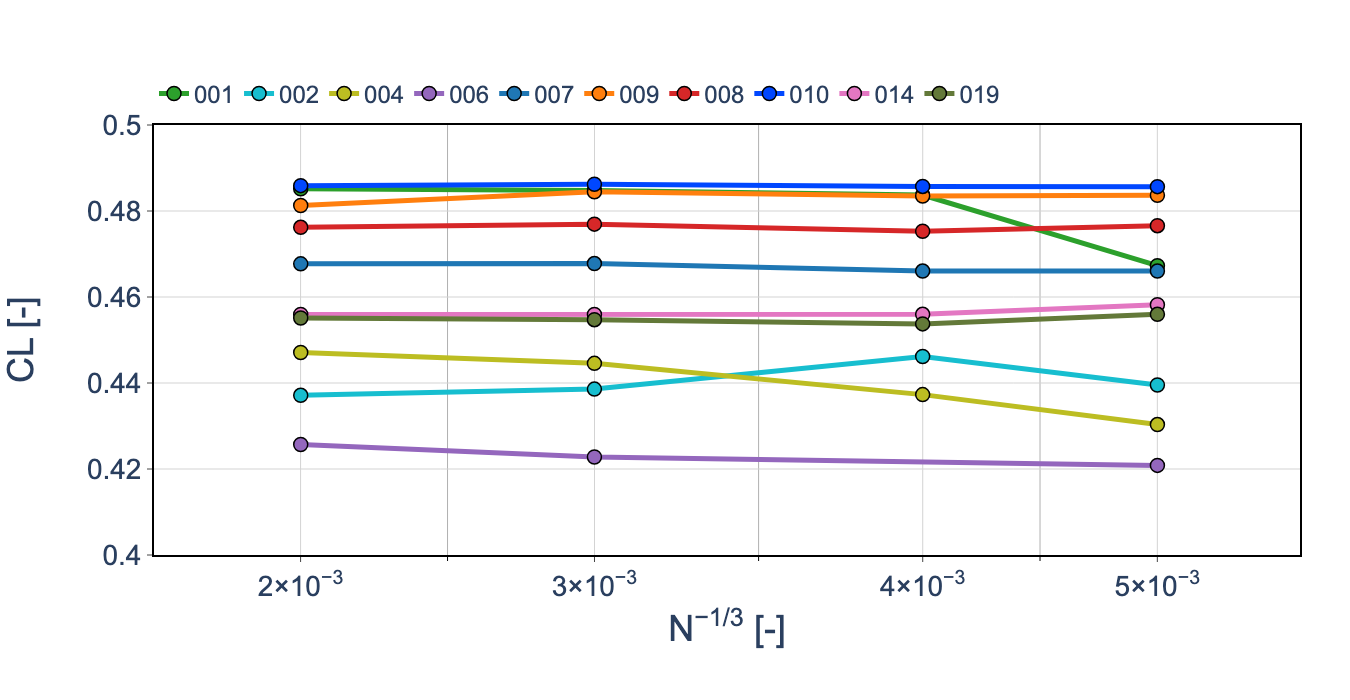
\includegraphics[trim={0cm 1cm 1cm 2.6cm}, clip, width=0.98\textwidth]{FIGURES/AERODYNAMIC/tc_naca0012_ae3932_cl_vs_n_all_roughness.png}
    \textbf{Grid-Level Values}
    \vspace{0.05cm}
\end{column}

\begin{column}{0.50\textwidth}
    \centering
    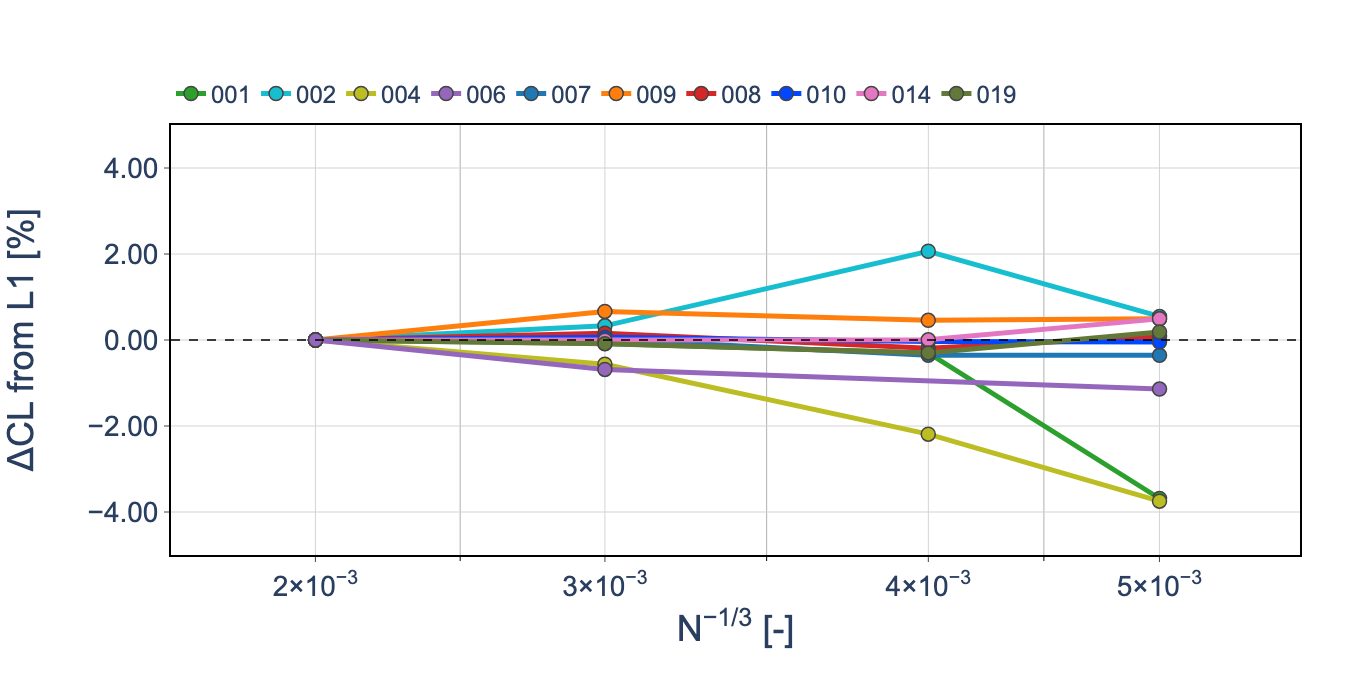
\includegraphics[trim={0cm 1cm 1cm 2.6cm}, clip, width=0.98\textwidth]{FIGURES/AERODYNAMIC/tc_naca0012_ae3932_cl_vs_n_all_roughness_relative_to_l1.png}
    \textbf{Relative to L1}
    \vspace{0.05cm}
\end{column}

\end{columns}

\vspace{-0.2cm}

\begin{block}{\scriptsize Observations}
\begin{itemize}
    \item At L1, the median lift coefficient is $C_L=0.4677$, with an IQR of $0.0262$ ($5.6\%$).
    \item Most submissions exhibit weak sensitivity to spatial grid refinement.
    \item Relative to L1, coarse-grid differences remain within approximately $4\%$ across the submissions.
\end{itemize}
\end{block}

\vspace{-0.1cm}
\vfill
{\tiny\textit{\textcolor{red}{*}IQR = interquartile range (75th percentile -- 25th percentile).}}

\end{frame}


% ============================================================
%  Aerodynamic Grid Convergence: CD
% ============================================================

\begin{frame}{\small  Drag Coefficient Grid Convergence}
\scriptsize
\vspace{-0.1cm}
\begin{columns}[T,onlytextwidth]

\begin{column}{0.50\textwidth}
    \centering
    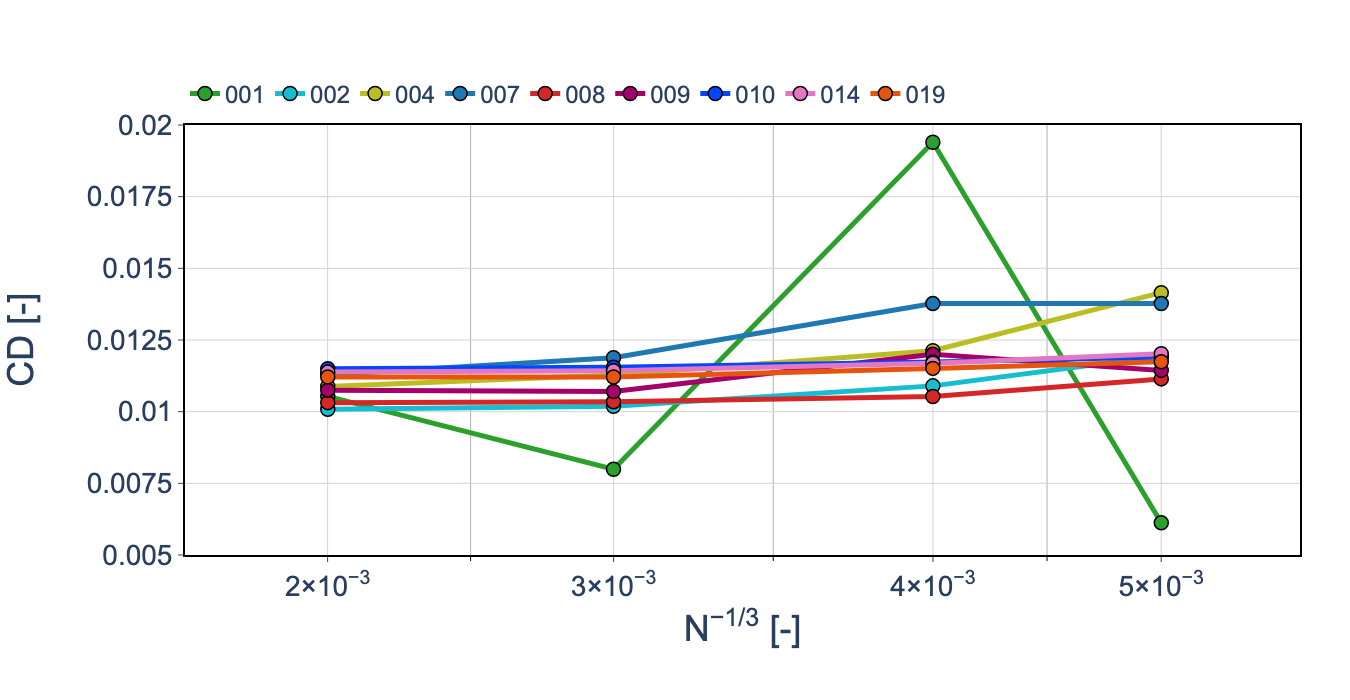
\includegraphics[trim={0cm 1cm 1cm 2.6cm}, clip, width=0.98\textwidth]{FIGURES/AERODYNAMIC/tc_naca0012_ae3932_cd_vs_n_all_roughness.png}
    \textbf{Grid-Level Values}
    \vspace{0.05cm}
\end{column}

\begin{column}{0.50\textwidth}
    \centering
    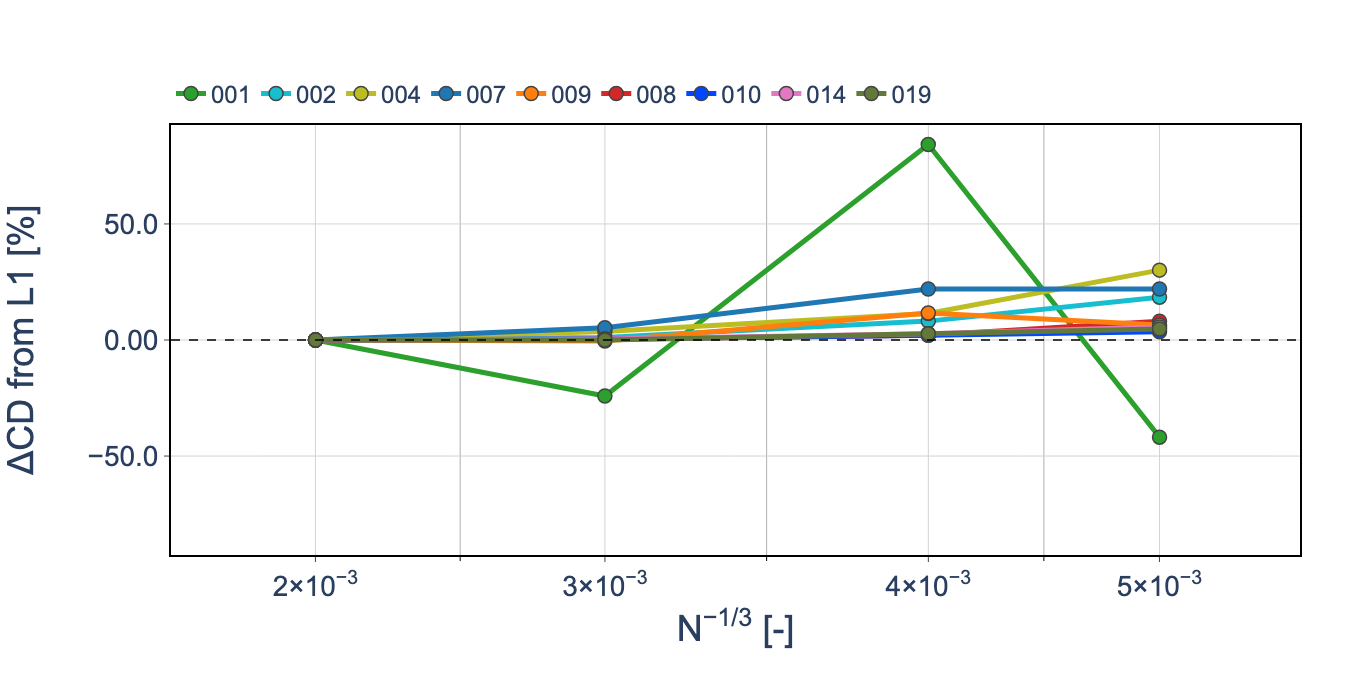
\includegraphics[trim={0cm 1cm 1cm 2.6cm}, clip, width=0.98\textwidth]{FIGURES/AERODYNAMIC/tc_naca0012_ae3932_cd_vs_n_all_roughness_relative_to_l1.png}
    \textbf{Relative to L1}
    \vspace{0.05cm}
\end{column}

\end{columns}

\vspace{-0.15cm}

\begin{block}{\scriptsize Observations}
\begin{itemize}
    \item At L1, the median drag coefficient is $C_D=0.01088$ (108.8 drag counts), with an IQR of 7.57 drag counts ($7.0\%$).
    \item $C_D$ exhibits the greatest sensitivity to spatial grid refinement, with coarse-grid deviations reaching approximately 30\% from L1.
    \item Most submissions show a consistent refinement trend.
\end{itemize}
\end{block}

\end{frame}


% ============================================================
%  Aerodynamic Grid Convergence: CM
% ============================================================

\begin{frame}{\small  Pitching Moment Grid Convergence}
\scriptsize

{\centering
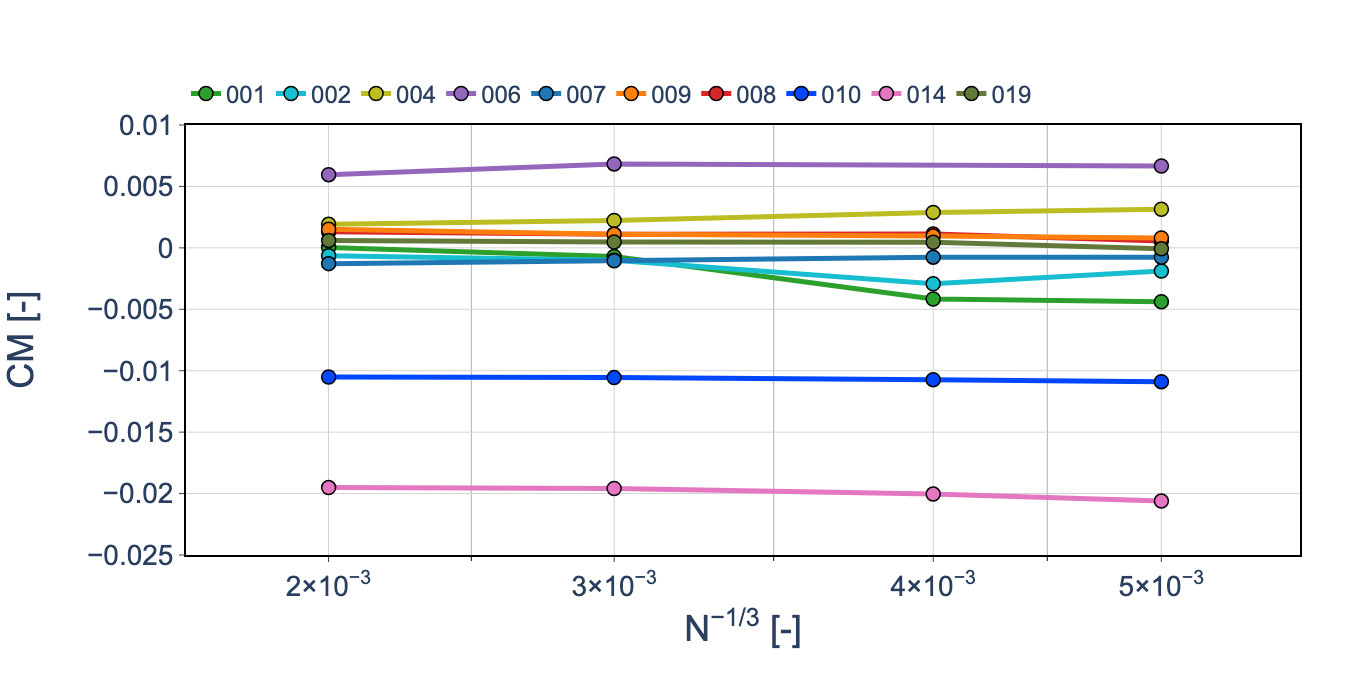
\includegraphics[trim={0cm 1cm 1cm 2.6cm}, clip, width=0.5\textwidth]{FIGURES/AERODYNAMIC/tc_naca0012_ae3932_cmy_vs_n_all_roughness.png}

\textbf{Grid-Level Values}
\vspace{0.05cm}
\par}

\vspace{-0.15cm}

\begin{block}{\scriptsize Observations}
\begin{itemize}
    \item At L1, the median pitching-moment coefficient is $C_M\approx2.50112\times10^{-5}$, with an IQR of $2.60\times10^{-3}$.
    \item Most submissions exhibit little variation in $C_M$ across the grid hierarchy.
\end{itemize}
\end{block}

\end{frame}


% ============================================================
%  Surface Pressure Distribution
% ============================================================

\begin{frame}{\small  Surface Pressure Distribution (L1)}
\scriptsize

\vspace{-0.15cm}

\begin{columns}[T,onlytextwidth]

\begin{column}{0.50\textwidth}
    \centering
    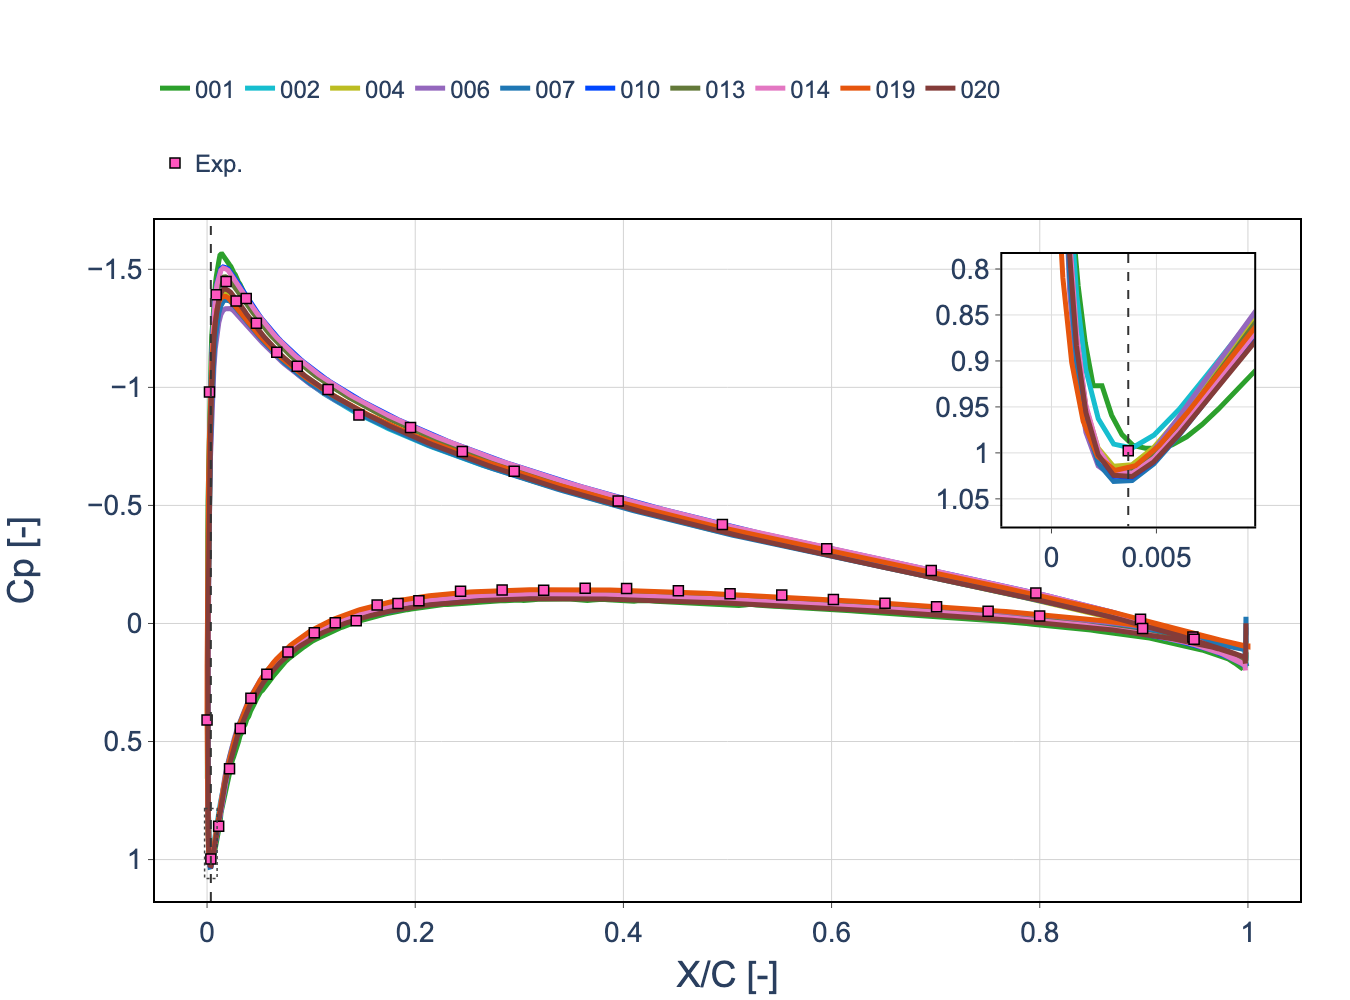
\includegraphics[trim={0cm 0cm 1cm 2.6cm}, clip, width=\textwidth]{FIGURES/AERODYNAMIC/tc_naca0012_ae3932_L1_cp_vs_x_slice_0p9144_all_roughness.png}
    \textbf{Cp vs X}
    \vspace{0.05cm}
\end{column}

\begin{column}{0.50\textwidth}
    \centering
    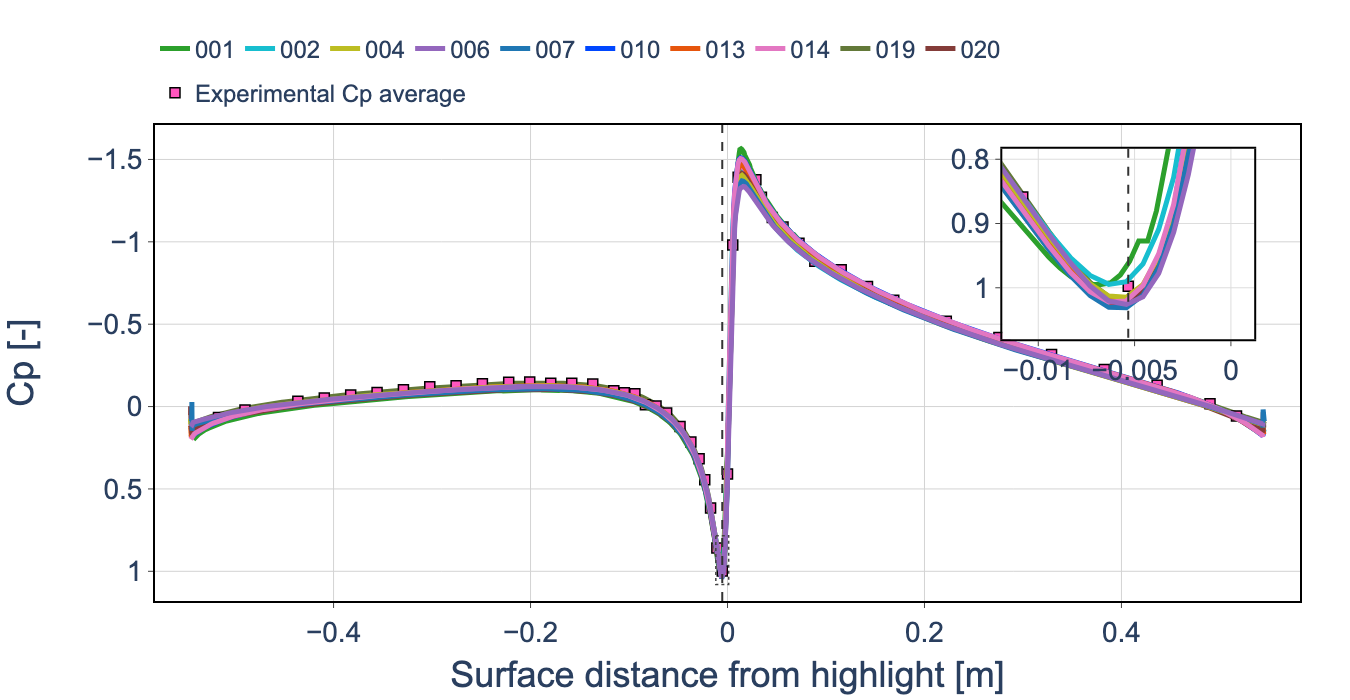
\includegraphics[trim={0cm 0cm 1cm 2.6cm}, clip, width=\textwidth]{FIGURES/AERODYNAMIC/tc_naca0012_ae3932_L1_cp_vs_s_slice_0p9144_all_roughness.png}
    \textbf{Cp vs s}
    \vspace{0.05cm}
\end{column}

\end{columns}

\vspace{-0.15cm}

\begin{block}{\scriptsize Observations}
\begin{itemize}
    \item The L1 $C_p$ distributions are tightly clustered and show good overall agreement with the experimental measurements.
    \item The largest code-to-code differences are localized near the leading-edge suction peak and stagnation region.
\end{itemize}
\end{block}

\end{frame}


% ============================================================
%  Aerodynamic Assessment Summary
% ============================================================

\begin{frame}{\small  Aerodynamic Assessment Summary}
\scriptsize

\begin{block}{\scriptsize Grid-Refinement Behavior}
\begin{itemize}
    \item $C_L$ and $C_M$ exhibit limited within-code sensitivity to grid refinement for most submissions.
    \item $C_D$ shows greater and less uniform grid sensitivity, including non-monotonic behavior for selected submissions.
    \item For most submissions, code-to-code differences exceed the changes produced by spatial refinement.
\end{itemize}
\end{block}

\vspace{0.15cm}

\begin{alertblock}{\scriptsize Aerodynamic Takeaway}
Overall, the aerodynamic predictions are well clustered, with L1 $C_p$ distributions showing good agreement with experiment. Among the integrated coefficients, $C_D$ exhibits the greatest sensitivity to spatial grid refinement.
\end{alertblock}

\end{frame}